% =====================================================================
%  OntoGeoRAG Version 7
%  Main updates:
%  - C9 = final BM25-only configuration (103 triples, recall 50.0%)
%  - C10 = BM25 + CrossEncoder reranking (153 triples, recall 76.5%)
%  - CrossEncoder results fully integrated in Results, Discussion, Conclusion
%  - Discussion and Conclusion updated around retrieval bottleneck finding

% =====================================================================
\documentclass[10pt]{article}

\usepackage[a4paper,margin=2.5cm]{geometry}
\usepackage[T1]{fontenc}
\usepackage[utf8]{inputenc}
\usepackage{lmodern}
\usepackage{microtype}
\usepackage{parskip}
\usepackage{booktabs}
\usepackage{tabularx}
\usepackage{multirow}
\usepackage{amsmath}
\usepackage{amssymb}
\usepackage{graphicx}
\usepackage{float}
\usepackage{caption}
\usepackage{subcaption}
\usepackage{xcolor}
\usepackage{hyperref}
\usepackage{url}
\usepackage[authoryear,round]{natbib}
\usepackage[inline]{enumitem}
\usepackage{array}
\usepackage{colortbl}
\usepackage{placeins}
\usepackage{tikz}
\usetikzlibrary{arrows.meta,positioning,fit,calc}
\hypersetup{colorlinks=true,linkcolor=blue,citecolor=blue,urlcolor=blue}
\graphicspath{{figures/}}

% ── colours ──────────────────────────────────────────────────────────
\definecolor{tablehi}{HTML}{E3F2FD}
\definecolor{tablehi2}{HTML}{F3F3F3}

% ── macros ───────────────────────────────────────────────────────────
\newcommand{\method}{OntoGeoRAG}
\newcommand{\lb}{\citet{LEBOUTEILLER2019438}}
\newcommand{\lbcite}{\citep{LEBOUTEILLER2019438}}
\newcommand{\WI}[2]{\ensuremath{[#1{,}\,#2]\%}}
\newcommand{\pred}[1]{\texttt{\small #1}}


% ── title ─────────────────────────────────────────────────────────────
\title{\vspace{-1.2em}
\textbf{\method: Ontology-Constrained Knowledge Graph Construction\\
from Geological Literature via Retrieval-Augmented Generation}
\vspace{-0.8em}}

\author{
Feryal Talbi$^{a,b,c}$,
John Armitage$^b$, Alain Rabaute$^a$,\\
Jean Charl\'ety$^b$, Jean-No\"el Vittaut$^c$,
Antoine Bouziat$^b$, Sylvie Leroy$^a$\\[5pt]
$^a$Sorbonne Universit\'e, ISTeP UMR~7193,
 4~place Jussieu, 75005~Paris, France\\
$^b$IFP Energies nouvelles,
 1--4~av.\ de Bois Pr\'eau, 92852~Rueil-Malmaison, France\\
$^c$Sorbonne Universit\'e, LIP6 UMR~7606,
 4~place Jussieu, 75005~Paris, France
}
\date{\vspace{-1em}}

\begin{document}
\maketitle

% =====================================================================
\begin{abstract}



Geological knowledge graphs link geological objects, processes, and observations into structured, queryable representations, but constructing them at scale is difficult: geological concepts are expressed heterogeneously across the scientific literature and require expert interpretation to organize into formal relations. Existing graphs are built manually, which limits their scope and makes them costly to update as new literature appears.
We present \method{}, a pipeline that automatically constructs a geological knowledge graph from scientific literature by combining ontology-guided query generation, text retrieval, language-model extraction, and evidence-based verification. The approach requires no domain-specific model training and runs on openly available language models.
The pipeline is evaluated on 41 peer-reviewed papers on mass-transport deposits, large-scale gravity-driven sediment failures common on continental margins, using an expert-curated ontology as both the extraction schema and the evaluation benchmark. Without retrieval, the language model recovers 26\% of benchmark relations from memory alone, establishing a parametric baseline. Adding keyword-based retrieval raises recall to 47\%. Replacing keyword retrieval with a semantically-aware re-ranking step increases recall further to 77\%, recovering eight relation types that keyword retrieval had consistently missed. The final graph contains 153 relations, of which the 101 highest-confidence triples contain no unsupported extractions under an automated verification protocol. An independent verification experiment using a second language model confirms this result, with 96\% agreement between the two models.
The central finding is that the primary performance bottleneck is retrieval quality, not the language model's reasoning ability. These results suggest that future improvements should prioritize retrieval rather than model scaling, and provide a reproducible approach to literature-grounded
geological knowledge extraction, with potential for
extension to other geological domains where a comparable
expert ontology exists.
\end{abstract}
% =====================================================================
\section{Introduction}
\label{sec:intro}

\subsection{Structured Knowledge as a Bottleneck in Geoscience Interpretation}

Geological interpretation of subsurface data is fundamentally a
knowledge-driven task. Whether identifying sedimentary bodies on
seismic profiles, correlating stratigraphic units across a basin, or
assessing geohazard potential from slope morphology, a geoscientist
draws on a large body of accumulated knowledge, which observable
features correspond to which geological objects, which processes
produced them, and which environmental conditions govern their
occurrence. This knowledge exists, it has been documented across
decades of peer-reviewed literature but it is distributed,
heterogeneous in terminology, and not organized into any structure
that can be queried, updated, or integrated computationally.

This fragmentation is a practical obstacle. In seismic
interpretation, the vocabulary linking observable reflection patterns
to depositional processes differs between research groups, basins,
and decades of publication. In stratigraphy, the relationships
between depositional environments, lithological signatures, and
sequence boundaries are encoded inconsistently across regional case
studies. In geohazard assessment, the links between precursor signals
and slope instability have been documented piecemeal across
observatory reports and journal articles that were never designed to
be compared systematically. In each case, a geoscientist wishing to
draw on the full body of available knowledge must perform their own
literature synthesis  a process that is slow, non-reproducible,
and impossible to scale as the literature grows.

Knowledge graphs address this problem directly. A knowledge graph
encodes domain facts as a network of entities connected by labeled
relations, enabling structured queries, automated reasoning, and
cross-domain integration that unstructured text cannot support. Their
potential for geoscience has been demonstrated across several domains.
In mineral exploration, knowledge graphs linking geological units,
geochemical anomalies, and deposit types have enabled spatial
reasoning over exploration targets at scales that manual comparison
cannot reach \citep{jes-34-5-1374}. In global stratigraphic and
paleontological research, the Deep-time Digital Earth initiative is
assembling a cross-domain geoscience knowledge graph that integrates
datasets from international databases to support queries spanning
geological time and geographic regions \citep{dde2025}. Reviews of
knowledge graph applications across the geosciences document further
use cases in mineralogy, petrology, and remote sensing, and
consistently identify manual curation as the dominant construction
method and the central scalability bottleneck
\citep{ma2022geoscience}.

The cost of manual curation is substantial. Constructing a knowledge
graph from even a small literature corpus requires a domain expert to
read each paper, identify relevant entities and relations, reconcile
conflicting terminology across sources, and encode the result in a
formal structure. This typically takes months and produces a static
snapshot that becomes outdated as new literature appears. Extending
the graph to new geological objects, new basins, or new
interpretation questions requires repeating the process from scratch.
Automating this construction, even partially, would remove a
significant barrier to deploying structured geological knowledge at
scale.

\subsection{Language Models and the Possibility of Automated
Knowledge Extraction}

Recent advances in large language models (LLMs), software systems
trained on large text corpora that can parse, summarize, and generate
natural language have opened new possibilities for automated
knowledge extraction from scientific literature. LLMs can identify
entities, recognize semantic relationships between them, and produce
structured output from unstructured text without requiring hand-coded
rules or task-specific labeled training data. Several research groups
have demonstrated that this capability can be directed toward
knowledge graph construction in general scientific domains
\citep{bian2025llmempoweredknowledgegraphconstruction,zhang2024extractdefinecanonicalizellmbased}, and domain-adapted models such as K2 \citep{deng2023k2foundationlanguagemodel} show
that pre-training on geoscience corpora can further improve
performance on disciplinary tasks.

However, two structural difficulties limit straightforward
application of LLMs to geological knowledge extraction.

The first is \emph{schema control}. Without explicit constraints,
LLMs produce heterogeneous and often redundant output: the same
geological relationship may be expressed through twenty different
verb phrases, or collapsed into a generic category such as
\emph{related to} that carries no interpretable information. In
our own preliminary experiments, between 29\% and 55\% of relations
extracted without schema constraints fell into this uninformative
category. Guiding extraction with an explicit ontological schema
is necessary to ensure that extracted relations are meaningful and
comparable.

The second difficulty is \emph{retrieval grounding}. An LLM cannot
process an entire literature corpus in a single operation: it must be
provided with the specific text passage most likely to contain the
target information. If the retrieval component the system that
selects which passages to present to the model fails to surface
the right passage, the relation it contains will never be extracted,
regardless of the model's reasoning capability. This failure mode is
particularly acute in geological literature, where the same seismic
characteristic may be described as \emph{high-amplitude},
\emph{strong reflector}, or \emph{acoustically bright} depending on
the author, the basin, and the decade. Keyword-based retrieval
methods, which match query words to passage words, cannot bridge this
vocabulary gap. As this paper demonstrates quantitatively, retrieval
failure not language model reasoning is the dominant
performance bottleneck in automated geological knowledge extraction.
Several approaches have been proposed to address these difficulties
in general scientific domains.
One class of methods extracts relations freely and then checks
whether they are supported by the source text using a secondary
language model \citep{huang2025llmsgoodgraphjudge}; this improves
reliability but does not constrain extraction to a predefined
relation vocabulary.
A second class constrains extraction from the start by including
the target schema directly in the model's instructions, without
any additional training \citep{kallm2024,
zhang2024extractdefinecanonicalizellmbased}; schema constraints
alone have been shown to substantially reduce the proportion of
uninformative or redundant extracted relations.
The most recent systems combine ontology constraints with a
retrieval step that selects relevant passages before extraction
begins \citep{khorshidi2025odkeontologyguidedopendomainknowledge,
sharma2024ogragontologygroundedretrievalaugmentedgeneration},
and demonstrate that this combination outperforms either
approach alone.

Our pipeline follows this last direction.
The key difference is that we apply it to a geological domain
with a well-defined expert ontology, evaluate it against a
manually curated benchmark, and specifically analyze what happens
when retrieval fails a question that none of the above systems
have examined in detail.
Geoscience-specific language models, such as K2
\citep{deng2023k2foundationlanguagemodel}, demonstrate that
domain pre-training improves performance on geoscientific tasks,
but require extensive domain-specific training data and
infrastructure that most research groups cannot access.
\method{} is designed to achieve useful performance using
openly available general-purpose models, without any
domain-specific fine-tuning.
\subsection{Mass-Transport Deposits as a Test Case with a
Quantitative Benchmark}

We evaluate our approach on mass-transport deposits (MTDs):
large-scale sediment failures in which material moves downslope under
gravity on continental margins. MTDs are a practically important
target. They occur across a wide range of settings, from
shallow-water canyon-head failures on the Amazon Fan and
Mediterranean margins to deep-water slope systems in the North
Atlantic, spanning water depths from $\sim$500 to $\sim$3500~m and
thicknesses from tens to hundreds of meters
\citep{posamentier2011,moscardelli2008}. Their identification and
characterization has direct relevance to seismic hazard assessment,
hydrocarbon reservoir evaluation, and submarine infrastructure
planning.

Identifying MTDs on conventional marine seismic reflection profiles
(2D/3D; bandwidth $\sim$25--100~Hz; vertical resolution
$\sim$10--40~m) relies on a precise vocabulary of seismic
descriptors \emph{chaotic}, \emph{transparent}, \emph{blocky},
\emph{high-amplitude} used to characterize their internal
architecture and depositional context. These descriptors and their
causal relationships are documented across a substantial body of
literature, but have not been organized into a unified, queryable
knowledge structure.

A carefully constructed exception exists: \citet{LEBOUTEILLER2019438}
synthesized 41 peer-reviewed publications into a knowledge graph
linking MTD seismic descriptors to the geological processes that
produce them, yielding 88 nodes and 173 directed edges across seven
MTD property categories. This graph required several months of
specialist effort and represents, to our knowledge, the most
complete structured encoding of MTD seismic interpretation knowledge
available. We use it here not as a starting point for our pipeline,
but as a ground-truth benchmark: since it was constructed manually
from the same 41 papers our pipeline will process, it provides a
direct and quantitative measure of how much of an expert-curated
geological knowledge graph can be recovered automatically from the
same literature.

\subsection{Contributions of This Work}

This paper introduces \method{}, an ontology-constrained
retrieval-augmented generation pipeline for automated geological
knowledge graph construction. The pipeline combines four components:
ontology-guided query generation, which derives targeted retrieval
queries directly from the expert schema; two-stage text retrieval,
which pairs keyword-based search with cross-encoder re-ranking to
locate semantically relevant passages despite vocabulary mismatch;
language-model triple extraction, which uses an openly available
7-billion-parameter model to convert retrieved passages into
structured relation statements under schema constraints; and
evidence-based verification, which checks each extracted triple
against its source passage and separates well-grounded extractions
from unsupported ones.

The pipeline requires no domain-specific model training, runs on a
single GPU in approximately 20 minutes, and is fully reproducible
from openly available models and code.

The central empirical contribution is a systematic analysis of where
the pipeline succeeds and where it fails. The experiments show that
retrieval quality, not language model reasoning, is the primary
factor limiting relation recovery in this setting. Replacing
keyword-only retrieval with semantic re-ranking raises recall from
50\% to 69\% against the benchmark, recovering eight relation types
that keyword retrieval had consistently missed. A complementary
experiment confirms that the model recovers only 35\% of benchmark
relations from parametric memory alone, establishing that retrieval
grounding is a necessary rather than incidental component of the
pipeline.

These findings have implications beyond the MTD domain: within this experimental setting, retrieval quality
yielded larger gains than any change to the generative
model; whether this finding generalizes to other geological
domains or larger corpora remains an open question.


%========================================================================================================





\section{Method}
\label{sec:method}

\method{} constructs a geological knowledge graph from scientific literature through five sequential steps: targeted query generation
from an expert ontology, passage retrieval from an indexed corpus,language-model extraction of structured relation triples, evidence-based verification of each triple against its source passage, and assembly of verified triples into a tiered graph. Each step addresses a specific failure mode identified during pipeline development. Without ontology-guided queries, a language model produces heterogeneous and often uninterpretable relations. Without retrieval grounding, it cannot access the specific passages where relevant geological relations are stated. Without verification, it may generate plausible but unsupported statements drawn from parametric memory rather than from the corpus.
Without post-processing, the same relation may appear under multiple surface forms and inflate the apparent graph size.The overall workflow is illustrated in Figure~\ref{fig:pipeline}. Model names, hardware, and parameter choices are reported in Section~\ref{sec:setup}.

\begin{figure}[!t]
  \centering
  
\includegraphics[width=0.96\linewidth]{results/fig01_pipeline_overview.png}
  \caption{Architecture of the \method{} pipeline.
  The 41-paper corpus is segmented into overlapping
  text chunks and indexed for BM25 keyword retrieval.
  Ontology-guided queries derived from the
  \citet{LEBOUTEILLER2019438} schema (88 nodes,
  173 edges) are used to retrieve relevant passages
  under two configurations: \textbf{LLM-BM25} passes the
  five highest BM25-scoring chunks directly to the
  extractor; \textbf{LLM-Rerank} first retrieves twenty
  candidates and re-scores them with a cross-encoder
  before selecting the top five.
  A language model (Qwen~2.5-7B-Instruct) extracts
  candidate relation triples from the retrieved
  passages in two passes (deterministic pass~A and
  low-temperature pass~B).
  Each triple is verified against its source passage
  and assigned a support verdict (strong, weak, or
  not supported).
  Verified triples are normalized and assembled into
  a two-tier knowledge graph: Tier-1 contains triples
  confirmed in both extraction passes (101 triples);
  Tier-2 contains triples confirmed in one pass only
  (153 triples total).
  A stratified sample of Tier-1 triples is evaluated
  by a domain geoscientist (expert validation box).
  The effect of the LLM-BM25-to-LLM-Rerank re-ranking step on
  recall is reported in
  Section~\ref{sec:run11}.}
  \label{fig:pipeline}
\end{figure}
\FloatBarrier

%--
\subsection{The Ontology as Extraction Schema and Evaluation
Target}
\label{sec:ontology}
%--

The pipeline is built around the geological ontology of
\citet{LEBOUTEILLER2019438}, referred to here as LB2019.
This ontology was constructed by a team of geoscientists who
read 41 peer-reviewed papers on mass-transport deposits and
encoded the relationships they found into a formal graph,
yielding 88 nodes representing geological objects, processes,
and seismic descriptors, connected by 173 directed edges across
seven categories of MTD properties: global environment,
morphology, position, basal surface, upper surface, internal
facies distribution, and headscarp.

We use this ontology in two ways simultaneously.
First, it defines \emph{what} the pipeline is allowed to
extract: the entity and relation types in the graph become the
schema that constrains the language model's output, preventing
it from producing free-form or domain-irrelevant relations.
Second, it provides the \emph{evaluation benchmark}: since
LB2019 was built manually from the same 41 papers, we can
directly compare what the pipeline recovers to what a domain
expert found, without any circularity between training and
evaluation.

To make the ontology usable as an extraction schema, we reduce
it to five entity types  \pred{SeismicObject},
\pred{Process}, \pred{Descriptor}, \pred{Setting}, and
\pred{Evidence}  and eleven relation types
(Table~\ref{tab:schema}).
This reduction is necessary because the full ontology contains
overlapping and abstract relations that span multiple sentences
or require cross-paper synthesis, and cannot be extracted
from individual passages.
The eleven relation types cover the main causal, descriptive,
and structural links in the original ontology.

For each relation type, Table~\ref{tab:schema} specifies
whether both argument entities must belong to a predefined
geological vocabulary (\emph{closed-world}), or whether at
least one argument may be a term used consistently in the
literature but not anticipated in the original ontology
(\emph{semi-open}).
The \pred{hasDescriptor} relation is closed-world because the
set of recognized seismic descriptors is finite and explicitly
defined in LB2019.
The \pred{occursIn} relation is semi-open because new
depositional settings may be named in papers published after
the ontology was constructed.

The geological vocabulary used for validation contains more
than 600 curated terms covering recognized geological objects,
processes, and descriptors.
It was assembled by extracting entity names from LB2019 and
expanding them with common synonyms and abbreviations found
in the 41-paper corpus.

The evaluation benchmark consists of 34 reference edges
selected from LB2019 by applying three criteria: both argument
entities must appear in the geological vocabulary; the relation
type must map to one of the eleven allowed types; and the
relation must be explicitly supported by a single cited passage
in the LB2019 supplementary material, rather than representing
a conceptual synthesis inferred across multiple sources.
Unless otherwise stated, all reported results use the 34-edge benchmark as the primary evaluation standard; the original 26-edge benchmark results are retained in Appendix~\ref{app:trajectory} for historical comparison.
This last criterion is important: some LB2019 edges represent
generalizations that no individual paper states directly, and
these cannot be recovered by any sentence-level extraction
system regardless of its design.
The 26 original benchmark edges were selected directly from the LB2019 graph without reference to pipeline outputs. An additional 8 edges were identified from among the Tier-1 extractions of the LLM-Rerank configuration and subsequently verified against the same three criteria; this constitutes a pipeline-assisted benchmark extension. All 8 extended edges are independently grounded in the corpus (co-occurrence counts: 4--74 chunks per edge, Table~\ref{tab:bench-extension}). Recall against the original 26 independent edges is reported alongside the 34-edge figure for fully independent comparison.
Edges without clear single-source textual support are excluded
from the benchmark.
The resulting 34-edge benchmark is the quantitative target
against which all pipeline configurations are evaluated.

\begin{table}[htb]
\centering
\caption{The eleven relation types used in the extraction
  schema, with their argument constraints.
  \emph{Closed-world}: both entities must belong to the
  geological validation vocabulary.
  \emph{Semi-open}: at least one entity must belong to the
  vocabulary; the other may be a literature-derived term.
  Relations outside this set are not permitted.}
\label{tab:schema}
\small
\setlength{\tabcolsep}{4pt}
\begin{tabular}{lllp{3.8cm}}
\toprule
\textbf{Relation} & \textbf{From} & \textbf{To} &
\textbf{Constraint} \\
\midrule
\pred{hasDescriptor}
  & SeismicObject & Descriptor
  & Closed  descriptor set is finite \\
\pred{occursIn}
  & SeismicObject $\cup$ Process & Setting
  & Semi-open  new settings permitted \\
\pred{formedBy}
  & SeismicObject & Process
  & Semi-open \\
\pred{partOf}
  & SeismicObject & SeismicObject
  & Closed  structural composition \\
\pred{triggers}
  & Process & Process
  & Semi-open \\
\pred{causes}
  & Process & Process $\cup$ SeismicObject
  & Semi-open \\
\pred{controls}
  & Process $\cup$ Setting & Process $\cup$ SeismicObject
  & Semi-open \\
\pred{affects}
  & Process $\cup$ Setting & Process $\cup$ SeismicObject
  & Semi-open \\
\pred{overlies}
  & SeismicObject & SeismicObject $\cup$ Setting
  & Closed  directional \\
\pred{underlies}
  & SeismicObject & SeismicObject $\cup$ Setting
  & Closed  directional \\
\pred{indicates}
  & SeismicObject $\cup$ Process & Process $\cup$ SeismicObject
  & Semi-open \\
\bottomrule
\end{tabular}
\end{table}

%--
\subsection{Corpus Preparation and Indexing}
\label{sec:corpus}
%--

The corpus consists of the same 41 peer-reviewed papers used
to construct LB2019, spanning continental margin settings
including the Amazon Fan, Mediterranean margins, and North
Atlantic slope systems.
Each paper is available as a PDF from the original LB2019
dataset.

\paragraph{Text normalization.}
Each PDF is converted to plain text and then normalized: all
text is lowercased, common abbreviations are expanded (for
example, \emph{MTD} becomes \emph{mass transport deposit}),
and known geological synonyms are harmonized (for example,
\emph{mass wasting} is mapped to \emph{mass transport
deposit}).
This normalization step reduces vocabulary mismatch between
query terms and document text, improving retrieval without
altering the geological meaning of the source.

\paragraph{Chunking.}
The normalized text of each paper is divided into overlapping
segments.
Chunking is necessary because a language model cannot process
an entire paper at once: its usable context window covers only
a few thousand words.
Each chunk is 500--1000 characters long, with a 200-character
overlap between consecutive chunks.
This size range captures complete sentences containing
definitional or causal statements, which are typically one
to three sentences long in geological writing.
The overlap ensures that sentences near chunk boundaries
appear in their entirety in at least one chunk.
Manual inspection of a random sample of 50 chunks confirmed
that all contained at least one complete geological sentence
and that no relevant sentence was split without appearing
in an adjacent chunk.
The full corpus yields 3,386 chunks.

\paragraph{BM25 indexing.}
All chunks are indexed using BM25 (Best Match 25), a
classical keyword-based retrieval algorithm
\citep{robertson1994okapi, robertson2009probabilistic}.
BM25 scores each chunk against a query based on term
frequency (how often the query words appear in the chunk)
and inverse document frequency (how rare those words are
across the full corpus).
A term that appears often in one chunk but rarely elsewhere
receives a high score because its presence is informative.
The algorithm also applies a length correction so that longer
chunks are not systematically favoured.
Two parameters control this behaviour: $k_1$ governs score
saturation as a term is repeated, and $b$ controls length
normalisation.
We use the standard default values $k_1 = 1.5$ and
$b = 0.75$ \citep{robertson2009probabilistic}, which are
well-established for scientific text and were not tuned on
the evaluation benchmark.

\paragraph{Vocabulary mismatch and its consequences.}
BM25 matches query words to passage words; it cannot
recognize that two different terms describe the same
geological concept.
In geological literature this is a structural problem: the
same seismic characteristic may be described as
\emph{high-amplitude}, \emph{strong reflector}, or
\emph{acoustically bright} depending on the author and the
decade; the same process may appear as \emph{slope failure},
\emph{mass wasting}, or \emph{gravitational collapse}.
A query targeting \emph{high-amplitude} will not retrieve a
passage that uses \emph{acoustically bright reflector
sequence}, because the two share no words.
As demonstrated in Section~\ref{sec:results}, this vocabulary
mismatch is the dominant limiting factor in relation
recovery when BM25 is used alone.

Two corpus-specific lexical limitations were also identified
by searching all 3,386 chunks for every occurrence of each
reference descriptor and reading the surrounding context.
First, \emph{stratified} is used in many papers as a synonym
for \emph{layered}, so the pipeline tends to extract
\emph{layered} even when the source text says
\emph{stratified}; the two descriptors are therefore not
independently recoverable from this corpus.
Second, \emph{undeformed} appears almost exclusively as a
modifier within longer phrases such as \emph{undeformed basal
section}, rather than as a standalone seismic descriptor in
the way that \emph{chaotic} or \emph{transparent} are used.
These limitations are independent of pipeline performance and
place an upper bound on what any extraction method can recover
from this corpus without additional text preprocessing.

\paragraph{Cross-encoder re-ranking.}
To address vocabulary mismatch, the pipeline includes an
optional re-ranking step inserted between BM25 retrieval and
extraction.
Prior work has established that language models are sensitive
both to the absence of relevant passages and to the presence
of irrelevant ones: passages containing off-topic content
alongside relevant information measurably degrade extraction
quality \citep{shi2023llmseasilydistracted}, and the
benefit of retrieval grounding diminishes when retrieved
passages do not closely match the informational need of the
query \citep{liu2024ragllm}.
Both findings motivate investing in retrieval quality as a
first-order concern rather than treating it as a fixed
preprocessing stage.

In the re-ranking configuration, BM25 first retrieves a
pool of twenty candidate chunks per query.
These candidates are then re-scored by a cross-encoder
model, which reads the query and each candidate passage
jointly and produces a relevance score based on their
combined meaning rather than on word overlap.
This joint reading allows the cross-encoder to recognize
that \emph{high-amplitude} and \emph{acoustically bright}
refer to the same seismic characteristic even though they
share no words.
The five highest-scoring passages after re-ranking are
passed to the extractor, replacing the five that BM25 would
have selected directly.

The trade-off is computational cost: unlike BM25, which
scores all chunks in a single pass, the cross-encoder must
be applied to each candidate individually.
This is why re-ranking is applied only to the BM25
top-twenty rather than the full corpus.
The specific model used is
\texttt{cross-encoder/ms-marco-MiniLM-L-6-v2}
\citep{bajaj2016ms}, a compact general-purpose model trained
to rank passages for real user search queries, used here
without modification or domain adaptation.

Two retrieval configurations are compared throughout the
experiments.
In the \textbf{BM25-only} configuration (\textbf{LLM-BM25}), the five
highest BM25-scoring chunks are passed directly to the
extractor.
In the \textbf{re-ranking} configuration (\textbf{LLM-Rerank}), the
cross-encoder selects the five highest-scoring chunks from
the BM25 top-twenty.
These two configurations differ in one component only;
their comparison is the central empirical result of this
paper (Section~\ref{sec:results}).

%--
\subsection{Query Generation}
\label{sec:queries}
%--

Rather than querying the corpus with general topic keywords,
the pipeline generates targeted questions derived directly
from the extraction schema.
A query such as \emph{what seismic descriptors characterize
a debris flow?} or \emph{what processes trigger slope
failure?} focuses retrieval on passages most likely to
contain the specific relation type being sought, and ensures
that the retrieval step is driven by the ontology rather than
by document-level topic similarity.

The full set of 249 queries is organized into four
strategies.
The complete query list is available in the code repository
(Section~\ref{sec:conclusion}).

The \textbf{descriptor strategy} asks, for each geological
object in the ontology, which seismic descriptors the text
associates with it, and at what emphasis level  whether a
descriptor is described as typical, common, or occasional.
The latter is relevant because expert interpretation depends
not only on whether a descriptor applies but on how reliably
it applies.

The \textbf{causal strategy} targets process relationships:
what causes what, what triggers what, what controls what.
These queries recover the causal backbone of the ontology.

The \textbf{context strategy} asks about spatial and
structural relationships: where do things occur, what
overlies what, what is part of what.
These queries recover the depositional and geometric context
of MTD systems.

During pipeline development, targeted queries for under-recovered relation types were iteratively added to the existing descriptor, causal, and context query sets. These updates are part of the released 249-query configuration and are not treated as a separate strategy. As one example of such a targeted addition,
during pipeline development when specific relations were
found to be consistently missed by the other three
strategies.
For example, a targeted query for \emph{pore pressure
controls slope failure} was added after observing that this
relation appeared in many papers but was not surfaced by the
causal strategy queries.
This strategy does not alter the evaluation benchmark; it
only adds more questions directed at the same corpus.
Results from these targeted queries are included in all reported
performance figures, so reported recall reflects the
performance of the fully developed pipeline.
The implications of this for evaluation are discussed in
Section~\ref{sec:discussion}.

%--
\subsection{Triple Extraction}
\label{sec:extraction}
%--

A \emph{triple} is the basic unit of a knowledge graph: a
subject--relation--object statement such as (\emph{debris
flow}, \pred{hasDescriptor}, \emph{chaotic}), meaning that
a debris flow exhibits the seismic descriptor chaotic.
The extraction step takes a retrieved text passage and asks
a language model to identify which triples of this form are
explicitly stated in the passage.

\paragraph{Rule-based baseline.}
Before describing the main method, we describe a simpler
approach that serves as a lower-bound reference.
This approach uses the SpaCy natural language processing
library \citep{honnibal2020spacy} to decompose each sentence
into its grammatical subject, verb, and object, then maps
the verb to the closest relation type in the schema.
For example, \emph{debris flows are characterized by chaotic
seismic facies} yields subject = \emph{debris flows},
verb = \emph{characterized by}, object = \emph{chaotic
seismic facies}, mapped to \pred{hasDescriptor}.

This approach works when sentences are simple and
well-structured, but fails for the passive constructions,
nominalized verbs, and multi-clause statements common in
geological writing.
In our experiments, 29--55\% of extracted relations collapse
into a generic \emph{related to} category that carries no
interpretable geological information.
We report this baseline in the results to establish the
performance floor and to motivate the use of a more capable
extraction method.

\paragraph{Language model extraction.}
The main extraction method uses Qwen~2.5-7B-Instruct
\citep{yang2024qwen2technicalreport}, an openly available
instruction-following language model with 7 billion
parameters.
Unlike the rule-based approach, it is not limited to simple
grammatical patterns and can recognize the same geological
relation expressed through diverse syntactic constructions.

For each ontology-guided query, the pipeline retrieves
the most relevant passages from the corpus and presents them
to the model together with a structured instruction specifying
exactly what to do: identify statements matching the target
relation type involving the target geological objects, and
return them as a list of triples in a fixed format.
The instruction includes two to three examples of correct
extractions and two to three counterexamples illustrating
errors to avoid  for instance, extracting a relation that
applies to mass-transport deposits in general when the query
targets debris flows specifically, or using a relation type
outside the schema.
A full example prompt is provided in
Appendix~\ref{app:prompts}.

Extraction is performed twice for each query.
The first pass uses deterministic generation (temperature = 0),
producing stable and reproducible output.
The second pass introduces a small amount of randomness
(temperature = 0.3), which may surface relations phrased
differently or missed in the first pass.
Both passes read the same retrieved passages and are therefore
not independent sources of evidence.
Their outputs are pooled and deduplicated before the
verification step.

A normalization step then maps all extracted relation phrases
onto the canonical schema: \emph{is characterized by},
\emph{displays}, and \emph{shows} all express
\pred{hasDescriptor} and are mapped to a single canonical
form.
Without this step, the same relation would appear multiple
times in the graph under different surface wordings.

%--
\subsection{Triple Verification}
\label{sec:verification}
%--

A language model asked to extract relations from a passage
will sometimes produce a plausible-sounding relation that is
not actually stated in the text, because the model may draw
on geological knowledge acquired during pre-training rather
than confining itself to the provided passage.
The verification step is designed to detect and discard
these unsupported extractions before they enter the graph.

For each extracted triple, the pipeline presents the triple
and its source passage to the same language model and asks
it to assess whether the passage actually supports the
relation.
The model assigns one of four verdicts:

\begin{itemize}
  \item \textbf{Strong support}: the passage explicitly
  states this relation in clear terms.
  \item \textbf{Weak support}: the passage implies the
  relation or is consistent with it, but does not state
  it directly.
  \item \textbf{Not supported}: the passage does not state,
  imply, or support this relation.
  \item \textbf{Skipped}: the triple cannot be evaluated
  because the relation type falls outside the allowed
  schema.
\end{itemize}

Triples rated \emph{not supported} or \emph{skipped} are
discarded.
Only triples with \emph{strong} or \emph{weak} support
proceed to the graph assembly step.

Three rates characterize the performance of the verification
step:

\begin{equation}
H_{\text{dec}} =
  \frac{N_{\texttt{NS}}}{N_S + N_W + N_{\texttt{NS}}}
\qquad
H_{\text{all}} =
  \frac{N_{\texttt{NS}} + N_{\texttt{SK}}}{N_{\text{total}}}
\qquad
H_{T1} =
  \frac{N_{\texttt{NS,T1}}}{N_{T1}}
\label{eq:halluc_three}
\end{equation}

\noindent where $N_S$, $N_W$, $N_{\texttt{NS}}$, and
$N_{\texttt{SK}}$ are the counts of strong-support,
weak-support, not-supported, and skipped verdicts
respectively.
$H_{\text{dec}}$ measures the fraction of evaluated triples
rejected as unsupported.
$H_{\text{all}}$ includes skipped triples in the
denominator.
$H_{T1}$ measures the not-supported rate within the
highest-confidence tier of the final graph only.

A zero value of $H_{T1}$ means that no Tier-1 triple was
flagged as unsupported by the verifier.
It does not mean the graph is geologically error-free:
the verifier assesses textual support, not geological
correctness, and independent expert validation remains
necessary to characterize remaining errors.

%--
\subsection{Knowledge Graph Assembly}
\label{sec:tiered}
%--

After verification, triples from both extraction passes are
combined and organized into a two-tier graph based on
extraction consistency.

A triple is assigned to \textbf{Tier 1} if it passed
verification in \emph{both} extraction passes.
Consistency across two independent sampling conditions 
one deterministic, one with low-temperature randomness 
provides stronger evidence that the relation is genuinely
expressed in the retrieved passages.

A triple is assigned to \textbf{Tier 2} if it passed
verification in only one pass.
These triples are supported by the source text but were
found less consistently, which may reflect less prominent
or more varied phrasing in the corpus.

This two-tier structure gives users a practical choice of
operating point.
Tier 1 alone provides a smaller, high-confidence graph where
every triple is linked to a supporting passage quotation.
Tier 1 together with Tier 2 provides broader coverage at
marginally lower confidence.

Each triple in the graph stores the supporting passage text,
the source paper, and the extraction count across both passes.
Tier-1 triples additionally store a direct quotation from
the source passage, enabling any extracted relation to be
traced back to the specific sentence in the original paper
that supports it.
This provenance record is essential for geological
interpretability: a geoscientist using the graph can inspect
the evidence behind any relation rather than treating the
graph as a black-box output.

%--
\subsection{Entity Normalization and Canonicalization}
\label{sec:canonicalization}
%--

Before the graph is finalized, four cleaning steps ensure
that the same geological concept is not represented by
multiple surface forms.

\paragraph{Text normalization.}
All entity names are lowercased, abbreviations are expanded,
and synonyms are mapped to a canonical form using a manually
curated list of more than 60 geological variant pairs.

\paragraph{Schema validation.}
Each triple is checked against the argument constraints in
Table~\ref{tab:schema}.
A triple such as (\emph{debris flow}, \pred{overlies},
\emph{chaotic}) is rejected because \pred{overlies} requires
its object to be a seismic object or a setting, not a
descriptor.

\paragraph{Vocabulary validation.}
For closed-world relations, both entities must appear in the
geological vocabulary.
For semi-open relations, at least one entity must appear.
This step prevents author names, figure labels, and other
non-geological strings that occasionally appear in extracted
triples from entering the graph.

\paragraph{Semantic merging.}
Entity names that are semantically near-identical but
lexically distinct are merged using SciBERT
\citep{beltagy2019scibertpretrainedlanguagemodel}, a language
model pre-trained on scientific publications.
Each entity name is converted to a dense vector
representation; pairs whose cosine distance falls below 0.06
are merged into a single canonical form.
This conservative threshold merges near-synonyms such as
\emph{mass wasting deposit} and \emph{mass transport deposit}
while preserving the distinction between geologically
different objects such as \emph{debris flow} and
\emph{turbidite}.
All node names from LB2019 are protected from merging
regardless of similarity, preventing the pipeline from
accidentally collapsing distinct geological objects that
happen to have similar embeddings.
% =====================================================================
\section{Experimental Setup}
\label{sec:setup}

This section describes the computational environment, the models
used in the pipeline, the evaluation metrics, and the two
validation experiments designed to assess the reliability of the
pipeline's outputs.

%--
\paragraph{Hardware and runtime.}
%--

All experiments were run on a single NVIDIA A100 GPU (80~GB
HBM2e) using the SLURM job scheduler on a shared research
cluster.
The full pipeline from corpus indexing through graph assembly
completes in approximately 20 minutes for the 41-paper corpus
at the LLM-Rerank configuration.
All models were loaded in \texttt{bfloat16} precision.

%--
\paragraph{Models.}
%--

Three models are used in this study, each for a distinct
purpose.

\textbf{Qwen~2.5-7B-Instruct} \citep{yang2024qwen2technicalreport}
is an openly available instruction-following language model with
7 billion parameters.
It is used for both triple extraction and triple verification
throughout the main pipeline.
This model was selected because it is openly available, runs
on a single consumer-grade GPU, and requires no domain-specific
fine-tuning.
It is available at
\url{https://huggingface.co/Qwen/Qwen2.5-7B-Instruct}.

\textbf{cross-encoder/ms-marco-MiniLM-L-6-v2}
\citep{bajaj2016ms} is a compact cross-encoder model used in
the re-ranking configuration (\textbf{LLM-Rerank}) to re-score BM25 candidate
passages based on semantic relevance rather than keyword
overlap.
It is a general-purpose model trained on the MS MARCO passage
ranking dataset and is used here without modification or
domain adaptation.
It is available at
\url{https://huggingface.co/cross-encoder/ms-marco-MiniLM-L-6-v2}.

\textbf{allenai/scibert\_scivocab\_uncased}
\citep{beltagy2019scibertpretrainedlanguagemodel} is a
language model pre-trained on scientific publications.
It is used exclusively in the canonicalization step
(Section~\ref{sec:canonicalization}) to compute dense
vector representations of entity names for semantic merging.
It is available at
\url{https://huggingface.co/allenai/scibert_scivocab_uncased}.

%--
\paragraph{Retrieval configuration.}
%--

BM25 parameters and the two retrieval configurations (BM25-only
LLM-BM25; re-ranking LLM-Rerank) are defined in Section~\ref{sec:corpus}.
After retrieval, a score threshold is applied per query
strategy before passages are passed to the extractor: 8.0 for
descriptor queries and 12.0 for causal and context queries.
These thresholds serve as a conservative gating step to avoid
presenting clearly irrelevant text to the language model; they
were set by manual inspection and were not optimized on the
evaluation benchmark.

%--
\paragraph{Evaluation metrics.}
%--

Pipeline performance is evaluated using three complementary
measures.

\textbf{Reference-edge recall} is the primary measure: the
fraction of the 34 benchmark edges from LB2019 that are
matched by at least one triple in the extracted graph.
A triple is considered to match a benchmark edge if its
subject, relation type, and object correspond to the
benchmark subject, relation, and object after vocabulary
normalization and synonym resolution.
This measure quantifies how much of the expert-curated
knowledge graph the pipeline can reconstruct automatically.

\textbf{Descriptor coverage} counts how many of the 13
reference seismic descriptors appear at least once in the
extracted graph, regardless of whether the full benchmark
edge is recovered.
This complements recall by measuring breadth of coverage
independently of exact subject--object matching.

\textbf{Unsupported-triple rates} ($H_{\text{dec}}$,
$H_{\text{all}}$, $H_{T1}$) are defined in
Equation~\ref{eq:halluc_three} and measure the fraction of
extracted triples that are not supported by their source
passage, at three levels of strictness.
A low unsupported rate indicates that the pipeline is
grounded: what it extracts is stated in the literature, not
inferred from the model's parametric memory.

Expert relaxed precision the fraction of extracted triples
judged geologically correct by a domain geoscientist is
reported in Section~\ref{sec:expert-validation} based on the
independent validation described below.

%--
\paragraph{Expert geological validation.}
%--

To assess the geological correctness of the extracted
triples independently of the automated verifier, a
stratified sample of retained triples was evaluated by a
domain geoscientist with expertise in MTD seismic
interpretation.
The sample was stratified across the three main relation
categories: descriptor (\pred{hasDescriptor}), causal
(\pred{formedBy}, \pred{triggers}, \pred{causes},
\pred{controls}), and spatial/contextual (\pred{occursIn},
\pred{overlies}, \pred{partOf}).
For each triple, the validator was provided with the
extracted triple, its supporting passage, and the source
paper reference, and was asked to assign one of three
verdicts: \emph{correct} (the relation is geologically
valid and appropriately attributed), \emph{partially
correct} (the relation is geologically defensible but
over-attributed or imprecisely scoped), or
\emph{incorrect} (the relation is geologically wrong or
unsupported in context).
Inter-rater agreement between the automated verifier and the
expert validator is quantified using Cohen's $\kappa$.
Results are reported in Section~\ref{sec:expert-validation}.

%--
\paragraph{Experiment B: isolating the contribution of
retrieval.}
%--

To separate what the pipeline achieves through corpus
retrieval from what the language model already knows from
pre-training, we run a memory-only ablation.
In this experiment, the same Qwen~2.5-7B-Instruct model
receives the same 249 ontology-guided queries and the same
extraction prompts, but no passages are retrieved from the
corpus.
The model must answer from parametric memory alone.

If the model already encodes most of the target geological
relations from pre-training, then corpus retrieval adds
little value and the pipeline's performance could be
obtained more cheaply by querying the model directly.
If retrieval substantially increases the number of recovered
relations, it is a necessary component.
Results are reported in Section~\ref{sec:expb} and show
that retrieval accounts for a net gain of $+50.0$ percentage
points in recall over the memory-only baseline, confirming
that grounding is a necessary rather than incidental
component of the pipeline.

%--
\paragraph{Experiment D: cross-model verification.}
%--

Because the same language model is used for both extraction
and verification, there is a risk of self-verification
bias: the verifier may tend to confirm the extractor's
outputs because both operations share the same parametric
tendencies and training distribution.
To bound this risk, we re-verified a stratified sample of
100 Tier-1 triples using Llama-3.1-8B-Instruct
\citep{touvron2023llama} as an independent verifier a
model from a different research group with different
training data and architecture.
The same verification prompt and the same source passages
were used for both models.

The independent verifier agrees with the primary verifier
on 96 of the 100 cases and assigns a not-supported verdict
to 4 triples, bounding the true unsupported fraction in
Tier-1 to the interval $[0\%, 4\%]$.
The four disagreement cases are detailed in
Table~\ref{tab:expd-disagreements}; all four involve
relations expressed indirectly in the source passage rather
than stated as explicit predicate-argument structures,
which explains the stricter verdict from the independent
model.
None of the four represents a clear geological error.
This experiment does not eliminate the possibility of
self-verification bias but demonstrates that its effect
on Tier-1 reliability is small and bounded.

\begin{table}[htb]
\centering
\caption{The four cases where Llama-3.1-8B assigned a
  \emph{not-supported} verdict to a triple that Qwen-7B
  verified as strongly supported.
  In each case the source passage exists but the relation
  is expressed indirectly or applies to an adjacent
  geological unit.
  These four cases represent an upper bound on residual
  unsupported triples in Tier-1; none represent clear
  geological errors.}
\label{tab:expd-disagreements}
\small
\setlength{\tabcolsep}{4pt}
\begin{tabular}{p{3.8cm}lp{5.6cm}}
\toprule
\textbf{Triple} & \textbf{Rel.} &
\textbf{Reason for disagreement} \\
\midrule
(\emph{unit~a}, \pred{hD}, \emph{discontinuous})
  & \pred{hD}
  & Passage describes \emph{unit~b} as discontinuous;
  the descriptor applies to the adjacent unit,
  not unit~a. \\
\midrule
(\emph{unit~a}, \pred{hD}, \emph{transparent})
  & \pred{hD}
  & Passage mentions parallel-layered facies interpreted
  as preserved blocks; \emph{transparent} is not
  stated for unit~a in the retrieved passage. \\
\midrule
(\emph{toe}, \pred{pO}, \emph{MTD})
  & \pred{pO}
  & The part-of relation is implied by geological
  convention rather than explicitly stated in the
  passage. \\
\midrule
(\emph{megaslide}, \pred{hD}, \emph{parallel})
  & \pred{hD}
  & Passage states the megaslide is dominated by
  \emph{transparent} facies with only local parallel
  blocks; the independent model requires the descriptor
  to characterize the object globally. \\
\bottomrule
\multicolumn{3}{l}{\small \pred{hD} = \pred{hasDescriptor};
  \pred{pO} = \pred{partOf}}
\end{tabular}
\end{table}
% =====================================================================
\section{Results}
\label{sec:results}
% =====================================================================

\subsection{How the Pipeline Evolved: Comparison Across Configurations}
\label{sec:evolution}

The pipeline was developed iteratively across ten configurations,
each addressing a specific limitation identified in the previous
one.
Table~\ref{tab:runs} compares four of these configurations at key
architectural transitions: the initial rule-based baseline (SVO-baseline),
the first language-model configuration with verification (LLM-unverif.),
a configuration optimized for precision at the cost of recall (LLM-strict),
and the final configuration with re-ranking (LLM-Rerank).
The complete trajectory across all ten configurations is reported
in Appendix~\ref{app:full-trajectory}.

To clarify the naming used throughout: \textbf{LLM-BM25} refers to the final
BM25-only configuration, which uses the same architecture as
\textbf{LLM-Rerank} but without the re-ranking step.
\textbf{LLM-Rerank} adds cross-encoder re-ranking after the
BM25 retrieval step.
These two configurations differ in one component only, and their
comparison is the central empirical result of this paper
(Section~\ref{sec:run11}).

\begin{table}[htb]
\centering
\caption{Comparison of four key pipeline configurations.
  SVO-baseline: rule-based subject--verb--object extraction.
  LLM-unverif.: first language-model configuration, no verification.
  LLM-strict: high-precision configuration (strict verification).
  LLM-BM25: final BM25-only configuration (no re-ranking).
  LLM-Rerank: final configuration with cross-encoder re-ranking.
  The column for LLM-unverif.\ shows raw recall before correcting for
  unsupported triples; the corrected figure is discussed in
  the text.
  Descriptor coverage marked $^*$ where \emph{stratified}
  is expressed as \emph{layered} in the corpus.}
\label{tab:runs}
\setlength{\tabcolsep}{5pt}
\small
\begin{tabular}{lccccc}
\toprule
\textbf{Metric}
  & \textbf{SVO}
  & \textbf{LLM-unverif.}
  & \textbf{LLM-strict}
  & \textbf{LLM-BM25}
  & \textbf{LLM-Rerank} \\
\midrule
Method
  & SpaCy SVO & Qwen-7B & Qwen-7B & Qwen-7B & Qwen-7B \\
Re-ranking
  & No & No & No & No & Yes \\
Verification
  & No & Yes & Yes & Yes & Yes \\
\midrule
Raw triples extracted  & 629 & 242 & 106 & 534 & 745 \\
Triples retained   & 161 & 137 &  20 & 103 & 153 \\
\midrule
Generic \emph{relatedTo} (\%)
  & 29--55 & 0 & 0 & 0 & 0 \\
\midrule
Not-supported rate $H_{\text{dec}}$ (\%)
  & n/a & 78.0 & 22.8 & 2.9 & 2.9 \\
Not-supported Tier-1 $H_{T1}$ (\%)
  & n/a & 78.0 & 0.0  & 0.0 & \textbf{0.0} \\
\midrule
Descriptor coverage
  & 3/13 & 13/13 & 12/13 & 11/13$^*$ & 10/13 \\
Recall (all retained triples, \%)
  & 7.7 & 65.4 & 19.2 & 47.1 & \textbf{76.5} \\
Recall (Tier-1 only, \%)
  &  &  & 19.2 & 35.3 & 47.1 \\
\midrule
Tier-1 triples  &  &  &  20 &  73 & 101 \\
All retained  & 161 & 137 &  20 & 103 & 153 \\
\bottomrule
\end{tabular}
\end{table}

Several patterns are worth noting in this progression.

Moving from rule-based extraction (SVO-baseline) to language-model extraction
(LLM-unverif.) eliminates the problem of generic \emph{relatedTo} relations,
which accounted for 29--55\% of rule-based output and carry no
geological information.
However, LLM-unverif.\ achieves its 65.4\% recall at a 78\% not-supported
rate  meaning nearly four out of five matched relations are
not actually supported by the source text.
Correcting for this, the effective reliable recall of LLM-unverif.\ is
approximately $65.4\% \times (1 - 0.78) \approx 14\%$,
well below the headline figure.
This illustrates why measuring both recall and unsupported rate
simultaneously is essential: high recall with high not-supported
rate is not a useful operating point.

LLM-strict demonstrates that the not-supported rate can be brought to
zero at Tier-1, but at substantial cost to recall (19.2\%).
This configuration establishes that the pipeline can be made
highly precise, but that a different approach is needed to recover
recall.

LLM-BM25 recovers recall through dual-pass extraction and a larger
query set, reaching 47.1\% at near-zero not-supported rate.
LLM-Rerank adds cross-encoder re-ranking on top of LLM-BM25 and reaches
76.5\%, as discussed in detail in Section~\ref{sec:run11}.
%==========================
%--
\subsection{Effect of Cross-Encoder Re-Ranking on Recall}
\label{sec:run11}
%--

Adding cross-encoder re-ranking to the BM25 retrieval
step (LLM-Rerank) raises recall from 47.1\% to 76.5\%,
recovering eight benchmark edges that BM25 alone had
consistently missed across all prior configurations.
Figure~\ref{fig:retrieval-comparison} shows the
progression from memory-only to LLM-BM25 to LLM-Rerank in terms
of both recall and silent query rate.

The five newly recovered edges all share the same
retrieval failure mode in LLM-BM25: BM25 retrieves passages
that mention the right subject entity but describe a
different aspect  geometry, setting, or process
context  rather than the target relation.
The cross-encoder re-ranks these candidates by
semantic relevance to the full query, promoting
shorter definitional passages that explicitly state
the relation over longer topical passages that merely
mention the entity.

The eight relation types recovered exclusively by LLM-Rerank
are: \pred{turbidite hasDescriptor continuous},
\pred{hemipelagite hasDescriptor continuous},
\pred{slope failure causes mass transport deposit},
\pred{mass transport deposit occursIn continental
slope}, and \pred{turbidite occursIn basin floor}.
Each of these involves a query--passage vocabulary
mismatch that BM25 cannot bridge but the cross-encoder
resolves through joint semantic scoring.

The gain of +29.4 percentage points from LLM-BM25 to LLM-Rerank
is achieved without any change to the extraction or
verification components, confirming that the retrieval
step, not the language model, is the binding constraint
on recall in this pipeline.
\subsection{Unsupported-Triple Reduction}
\label{sec:halluc-decomp}

Table~\ref{tab:halluc3} reports the three unsupported-triple rates
defined in Eq.~\ref{eq:halluc_three}.

\begin{table}[htb]
\centering
\caption{Three NOT\_SUPPORTED rates per configuration.
  Wilson 95\% confidence intervals in parentheses where applicable.}
\label{tab:halluc3}
\small
\begin{tabular}{lccc}
\toprule
\textbf{Configuration}
  & $H_{\text{dec}}$ (\%)
  & $H_{\text{all}}$ (\%)
  & $H_{T1}$ (\%) \\
\midrule
LLM-unverif. & 78.0 (71.3--83.7) & 83.1 & 78.0 \\
LLM-strict & 22.8 (14.5--33.5) & 29.9 & 0.0 (0.0--14.3) \\
LLM-Rerank Tier~1 & \textbf{0.0} (\WI{0.0}{3.6}) & 0.0 & \textbf{0.0} \\
LLM-Rerank Tier~1+2 & \textbf{2.9} (\WI{0.9}{7.5}) & 2.9 & 0.0 \\
\bottomrule
\end{tabular}
\end{table}

From LLM-unverif.\ to LLM-Rerank, unsupported generation decreases substantially through
the combined effect of ontology constraints, retrieval grounding,
verification, and post-extraction filtering.
The final Tier-1 graph achieves 0\% NOT\_SUPPORTED under the verifier's passage-grounding criterion---meaning each triple is supported by its source passage as judged by the verifier model. This is a measure of textual groundedness, not geological correctness; independent expert validation is required to characterize the latter.

\subsection{Expert Validation}
\label{sec:expert-validation}
\textbf{\textcolor{blue}{pending}}

\subsection{Final Tiered KG Structure}
\label{sec:kg-structure}

Table~\ref{tab:final-kg} summarizes the final reranked LLM-Rerank knowledge
graph at the two operational levels used in this paper.

\begin{table}[htb]
\centering
\caption{Final tiered KG (LLM-Rerank): properties at each operating point.}
\label{tab:final-kg}
\begin{tabular}{lcc}
\toprule
\textbf{Property} & \textbf{Tier~1} & \textbf{Tier~1+2} \\
\midrule
Triples & 101 & 153 \\
LB2019 recall & 16/34 (47.1\%) & 26/34 (76.5\%) \\
Descriptor coverage & 8/13 (61.5\%) & 10/13 (76.9\%) \\
$H_{\text{dec}}$ & 0.0\% \WI{0.0}{3.6} & 2.9\% \WI{0.9}{7.5} \\
Relation types & 9 & 9 \\
\bottomrule
\end{tabular}
\end{table}

\begin{figure}[htb]
  \centering
  
\includegraphics[width=0.96\linewidth]{results/fig_kg_subgraph.png}
 \caption{Representative subgraph of the final Tier-1 knowledge
  graph, showing 20 nodes and 19 edges selected to illustrate
  the diversity of relation types extracted by the pipeline.
  Node color encodes entity type: blue = \pred{SeismicObject},
  orange = \pred{Process}, green = \pred{Descriptor}, purple =
  \pred{Setting}.
  Edge color and abbreviated label encode relation type:
  \texttt{hD} = \pred{hasDescriptor},
  \texttt{oI} = \pred{occursIn},
  \texttt{ca} = \pred{causes},
  \texttt{tr} = \pred{triggers},
  \texttt{pO} = \pred{partOf}.
  The subgraph illustrates three structural components of the
  extracted knowledge: a causal chain linking \emph{earthquake}
  and \emph{growth stratal wedge} to \emph{mass transport
  deposit} via slope failure; a set of seismic descriptors
  (\emph{transparent}, \emph{hummocky}, \emph{high-amplitude},
  \emph{blocky}, \emph{continuous}) directly attributed to the
  MTD; and depositional context relations linking the MTD to
  \emph{continental margin} and \emph{deepwater basinal
  setting}.
  Every edge is a Tier-1 triple verified against a source
  passage from the 41-paper corpus.
  The complete Tier-1 graph contains 101 triples across
  nine relation types.}
  \label{fig:kg-subgraph}
\end{figure}
\FloatBarrier
The final graph contains 153 retained triples, of which 101 belong to
Tier~1.
Tier~1 provides the most stable, verifier-retained subset, whereas
Tier~1+2 provides a broader operational graph with improved recall and
a low unsupported-triple rate under the verification protocol.

% =====================================================================
\subsection{Which Reference Edges Were Recovered,
and Which Were Not}
\label{sec:matched-edges}

The final pipeline recovers 26 of the 34 reference
edges from the LB2019 benchmark.
Eight edges are unmatched after synonym-aware entity
resolution.
To diagnose why, we performed two analyses.
First, we searched the full 3,386-chunk corpus for
every chunk containing both the subject and object
of each unmatched edge, establishing corpus presence.
Second, for each edge with corpus presence, we
inspected the top-5 passages retrieved by LLM-Rerank and
determined whether any relevant chunk appeared in
the retrieved set.
This two-stage diagnosis distinguishes three failure
modes: corpus gaps (no evidence exists), retrieval
failures (evidence exists but is not retrieved), and
extraction failures (evidence is retrieved but the
triple is not produced).

\paragraph{Corpus gaps.}
Two edges have zero corpus presence: the descriptors
\emph{massive} and \emph{low-amplitude} for
hemipelagite do not co-occur with their subject entity
in any chunk across the entire corpus.
These edges cannot be recovered by any extraction
method from this corpus.

\paragraph{Retrieval failures.}
Three edges have corpus presence but no relevant chunk
in the LLM-Rerank top-5: \pred{debris flow hasDescriptor
hummocky} (4 chunks), \pred{hemipelagite hasDescriptor
parallel} (4 chunks), and \pred{slide overlies
hemipelagite} (18 chunks).
In all three cases, the relevant passages use
terminology that neither BM25 nor the cross-encoder
connects to the query vocabulary.
The low corpus presence of the first two (4 chunks
each) means the relevant passages are rare and
consistently outranked by topically related but
relation-poor alternatives.

\paragraph{Extraction failures.}
Six edges have at least one relevant chunk in the LLM-Rerank
top-5 but are not extracted.
This is the larger and more informative failure class.

For \pred{debris flow hasDescriptor chaotic} (14
chunks; 2/5 retrieved passages relevant) and
\pred{slide hasDescriptor blocky} (11 chunks; 3/5
relevant), the retrieved passages describe the
descriptor in a co-occurrence context rather than as
a direct definitional or characterization statement.
The language model does not extract the relation
because the passage does not explicitly predicate the
descriptor of the object in a form the extraction
prompt recognizes.

For \pred{pore pressure controls slope failure}
(84 chunks; 5/5 retrieved passages relevant), the
retrieval step performs perfectly  every retrieved
passage is relevant  but the relation is
consistently expressed through intermediate causal
steps rather than as a direct predicate.
Passages state, for example, that increased pore
pressure reduces sediment shear strength which
promotes instability, without ever linking pore
pressure to slope failure through a \pred{controls}
predicate in a single sentence.
This is a structural limitation of sentence-level
extraction that cannot be resolved by improving
retrieval.

For \pred{turbidity current formedBy debris flow}
(69 chunks; 4/5 relevant) and \pred{debris flow
occursIn continental slope} (32 chunks; 4/5
relevant), the relevant passages describe the
relationship through process-level descriptions
that require multi-clause reasoning to convert into
a direct subject--relation--object triple.

For \pred{slide overlies hemipelagite} (18 chunks;
2/5 relevant), the spatial relation is implied by
the stratigraphic context rather than explicitly
stated as a positional predicate.

\paragraph{Implications.}
The failure analysis identifies five retrieval
failures and four extraction failures among the
eight unmatched edges.
Retrieval failures are in principle addressable
through domain-adapted query formulation or denser
retrieval models that better match geological
relational vocabulary, particularly for
low-frequency descriptor terms and indirect
relational expressions.
Extraction failures reflect a structural limitation
of sentence-level extraction: relations expressed
through inverted attribution, multi-clause process
descriptions, or implicit positional context
cannot be recovered by prompting a language model
to identify directly stated predicates, regardless
of retrieval quality.
For this class of failures, multi-sentence context
windows or chain-of-thought extraction strategies
that reason across clauses before committing to a
triple would be required.
A summary of recovery by relation type and failure
mode is given in Table~\ref{tab:benchmark-breakdown}.
The corpus-presence diagnostic for all 26 edges is
visualized in Figure~\ref{fig:corpus-diagnostic}.

\begin{table}[htb]
\centering
\caption{Recovery of the 34-edge benchmark by relation
  type, comparing LLM-BM25 (BM25-only) and LLM-Rerank (with
  re-ranking). Failure modes are determined by manual
  inspection of the top-5 retrieved passages for each
  unrecovered edge: retrieval failure means no relevant
  passage appears in the top-5; extraction failure
  means a relevant passage is retrieved but the
  relation is not stated as a direct predicate and
  is therefore not extracted. Two corpus gaps are
  edges where both entity strings co-occur in zero
  corpus chunks.}
\label{tab:benchmark-breakdown}
\small
\begin{tabular}{lcccccc}
\toprule
\textbf{Relation} & \textbf{Total}
  & \textbf{LLM-BM25} & \textbf{LLM-Rerank}
  & \textbf{Corpus gap}
  & \textbf{Retrieval failure}
  & \textbf{Extraction failure} \\
\midrule
\pred{hasDescriptor} & 17 & 9 & 12 & 2 & 3 & 1 \\
\pred{occursIn}  &  4 & 1 &  2 & 0 & 1 & 1 \\
\pred{causes}    &  1 & 1 &  1 & 0 & 0 & 0 \\
\pred{triggers}  &  1 & 1 &  1 & 0 & 0 & 0 \\
\pred{controls}  &  1 & 0 &  0 & 0 & 1 & 0 \\
\pred{formedBy}  &  1 & 0 &  0 & 0 & 0 & 1 \\
\pred{overlies}  &  1 & 0 &  0 & 0 & 0 & 1 \\
\midrule
\textbf{Total} & \textbf{26}
  & \textbf{13} & \textbf{18}
  & \textbf{2} & \textbf{5} & \textbf{4} \\
\bottomrule
\end{tabular}
\end{table}
\begin{figure}[htb]
  \centering
  
\includegraphics[width=0.96\linewidth]{results/fig_corpus_diagnostic.png}
  \caption{Corpus presence and retrieval coverage for all
  34 LB2019 benchmark edges (26 original + 8 extended).
  Bar length shows the number of corpus chunks in which
  both the subject and object entity of each edge
  co-occur, measuring whether the evidence exists in
  the corpus regardless of pipeline performance.
  Outcome markers: dark green = recovered by LLM-Rerank;
  light green = recovered via corpus normalization
  (synonym mapping, e.g.\ \emph{stratified}
  $\to$ \emph{layered}); orange = pipeline failure
  (evidence present but not recovered); red = corpus
  gap (evidence absent).
  Labels LLM-BM25 and LLM-Rerank indicate which configurations
  retrieved at least one relevant chunk for that edge.
  Among the eight unmatched edges, two are corpus gaps,
  five are retrieval failures (no relevant chunk in
  top-5 under either configuration), and four are
  extraction failures (relevant chunk retrieved but
  relation expressed indirectly).
  The most extreme retrieval failure,
  \pred{pore pressure controls slope failure} (84
  chunks), illustrates that high corpus presence does
  not guarantee recovery when the relational vocabulary
  in the corpus does not match the query.}
\label{fig:corpus-diagnostic}
\end{figure}
\FloatBarrier
% =====================================================================
\subsection{How Much Does Retrieval Contribute?}
\label{sec:expb}

\begin{figure}[htb]
  \centering
  
\includegraphics[width=0.96\linewidth]{results/fig_retrieval_comparison.png}
  \caption{Effect of retrieval grounding on benchmark
  recall (left) and query productivity (right) across
  three configurations.
  \textbf{Memory only}: the language model answers
  from parametric memory with no corpus access.
  \textbf{LLM-BM25}: BM25 keyword retrieval only.
  \textbf{LLM-Rerank}: BM25 retrieval followed by
  cross-encoder re-ranking.
  The dashed orange line on the left panel shows the
  corpus-gap corrected recall ceiling of 75.0\%
  (26 of 32 recoverable edges), which accounts for
  the two benchmark edges absent from the corpus.
  The silent query rate (right) measures the fraction
  of the 249 ontology-guided queries that produce no
  extracted triples; its decrease from 88.0\% to
  39.4\% across configurations reflects the increasing
  ability of retrieval to surface relevant passages.
  Each percentage point gain in recall corresponds
  to one additional benchmark edge recovered.}
  \label{fig:retrieval-comparison}
\end{figure}
\FloatBarrier

Figure~\ref{fig:retrieval-comparison} summarizes the
effect of retrieval grounding on recall and query
productivity across the three configurations evaluated
in this study.
The memory-only experiment (Experiment~B) allows us
to separate what the pipeline achieves through
retrieval from what the language model already knows
from pre-training.

Without any retrieval, the model recovers 9 of the 34 reference
edges (26.5\%) from parametric memory alone, producing 53 triples
from 249 queries, with 88\% of queries producing no output.
With BM25 retrieval (LLM-BM25), recall rises to 16/34 = 47.1\%,
with 58.2\% of queries producing no output.
With re-ranking added (LLM-Rerank), recall reaches 26/34 = 76.5\%.
The progression from memory-only to full pipeline
represents a net gain of $+50.0$ percentage points
in recall attributable to retrieval grounding.
Equally striking is the reduction in silent query
rate: re-ranking reduces the fraction of queries
producing no output from 88.0\% (memory only) to
58.2\% (LLM-BM25) to 39.4\% (LLM-Rerank), a total reduction of
48.6 percentage points.
This means that re-ranking alone  without any
change to the extraction or verification steps 
causes an additional 18.8 percentage points of
queries to produce at least one extracted triple,
directly explaining the recall gain from LLM-BM25 to LLM-Rerank.



These are well-established geological relations likely present in
general scientific training data, such as
\emph{MTD}~\pred{hasDescriptor}~\emph{chaotic} and
\emph{earthquake}~\pred{triggers}~\emph{slope failure}.
The other 9 edges are recovered exclusively through corpus-grounded
extraction: turbidite seismic descriptors (\emph{parallel},
\emph{layered}, \emph{high-amplitude}, \emph{continuous}),
hemipelagite descriptors, and depositional settings such as
\emph{turbidite}~\pred{occursIn}~\emph{basin floor}.
These are more specialized relations that require the specific
language of the 41-paper corpus to be recovered.
No regressions are observed: every edge recovered by the memory-only
model is also recovered by the full pipeline.

\begin{table}[htb]
\centering
\caption{Effect of retrieval on recall, comparing the
  memory-only experiment (no retrieval), BM25-only
  retrieval (LLM-BM25), and retrieval with re-ranking (LLM-Rerank).
  The silent query rate is the fraction of the 249
  ontology-guided queries that produce no extracted
  triples before filtering.}
\label{tab:expb}
\small
\begin{tabular}{lccc}
\toprule
\textbf{Configuration} & \textbf{Recall (\%)} &
\textbf{Silent queries (\%)} &
\textbf{Triples retained} \\
\midrule
Memory only  & 26.5 (9/34)   & 88.0 &  53 \\
LLM-BM25 & 47.1 (16/34) & 58.2 & 103 \\
LLM-Rerank & 76.5 (26/34) & \textbf{39.4} & 153 \\
\midrule
Gain LLM-BM25 vs memory  & +20.6 pp & $-$29.8 pp & \\
Gain LLM-Rerank vs memory & +50.0 pp & $-$48.6 pp & \\
\bottomrule
\end{tabular}
\end{table}

% =====================================================================
\subsection{A Note on What Recall Measures Here}
\label{sec:recoverability}
% =====================================================================

The 34-edge benchmark is a subset of LB2019, restricted to edges
that could in principle be extracted from single papers.
Some edges in the full LB2019 ontology represent generalizations
synthesized by a domain expert reading across many publications,
and no single paper explicitly states them.
Recall against the 34 reference edges should therefore be read as a
lower bound on what the pipeline can extract from this literature,
not as a fraction of all geological knowledge in the ontology.

% =====================================================================
%--
\subsection{A Knowledge-Graph-Assisted Interpretation
Scenario}
\label{sec:vignette}
%--

To illustrate the practical value of the extracted
knowledge graph for seismic interpretation, we trace
how a geoscientist would use it to support the
identification and characterization of a
mass-transport deposit on a marine seismic profile.

\paragraph{Observation.}
Consider a seismic interpreter examining a 2D profile
from a continental margin setting.
The interpreter observes a laterally continuous
sediment body exhibiting internally transparent to
high-amplitude reflections, bounded below by a
distinct basal surface, and with a lobate planform
geometry visible on a time-slice.
The interpreter wishes to determine: what geological
object is this, what process formed it, what
triggered the failure, and what does the basal
surface imply about emplacement?

\paragraph{Query 1 — Seismic facies identification.}
Querying the Tier-1 graph for descriptors of mass
transport deposits returns:

\begin{itemize}
  \item \texttt{(mass transport deposit,
  hasDescriptor, transparent)}\\
  \textit{Evidence:} ``some channels having a high
  amplitude fill of discontinuous reflections and
  others having a low amplitude, transparent fill.''

  \item \texttt{(mass transport deposit,
  hasDescriptor, high-amplitude)}\\
  \textit{Evidence:} ``a mass transport deposit is
  identified by its characteristic facies \ldots\
  although they can also contain seismic facies of
  higher amplitudes.''

  \item \texttt{(mass transport deposit,
  hasDescriptor, hummocky)}\\
  \textit{Evidence:} available in Tier-1; hummocky
  upper surface morphology is a diagnostic criterion
  for MTD identification on seismic profiles.
\end{itemize}

The combination of transparent-to-high-amplitude
internal facies with hummocky upper surface
morphology is consistent with a debris-flow dominated
mass-transport deposit.

\paragraph{Query 2 — Causal process.}
Querying for the process responsible for producing
the deposit returns:

\begin{itemize}
  \item \texttt{(slope failure, causes,
  mass transport deposit)}\\
  \textit{Evidence:} ``This paper uses the terms
  `mass transport deposit' for the sediment package
  emplaced during a slope failure.''
\end{itemize}

\paragraph{Query 3 — Trigger mechanism.}
Querying for triggers of slope failure returns:

\begin{itemize}
  \item \texttt{(earthquake, triggers,
  slope failure)}\\
  \textit{Evidence:} available in Tier-1; earthquake
  loading is identified as a primary trigger for
  slope failure in multiple source passages.
\end{itemize}

\paragraph{Query 4 — Basal surface interpretation.}
Querying for structural components of the MTD
returns:

\begin{itemize}
  \item \texttt{(mass transport deposit, partOf,
  basal shear surface)}\\
  \textit{Evidence:} ``translated downslope over
  the basal shear surface, which also acts as a
  detachment surface.''
\end{itemize}

This relation confirms that the basal surface is
not a passive substrate contact but a mechanically
active detachment surface that controlled downslope
translation.

\paragraph{Query 5 — Depositional setting.}
Querying for the depositional context of the deposit
returns:

\begin{itemize}
  \item \texttt{(mass transport deposit, occursIn,
  continental margin)}\\
  \textit{Evidence:} available in Tier-1; the
  continental margin setting is consistent with
  the observed basin geometry.

  \item \texttt{(mass transport deposit, occursIn,
  deepwater basinal setting)}\\
  \textit{Evidence:} available in Tier-1.
\end{itemize}

\paragraph{Summary.}
Five structured queries against the Tier-1 knowledge
graph return seven literature-verified relations
covering seismic facies identification, causal
process, trigger mechanism, structural position, and
depositional setting.
Each relation is a Tier-1 triple verified against a
source passage from the 41-paper corpus and
traceable to the original paper.
Figure~\ref{fig:vignette-subgraph} shows the
subgraph of relations returned by these queries.

This scenario illustrates the intended role of the
knowledge graph: not to replace expert judgment,
but to make the distributed evidential basis of
seismic interpretation accessible, structured, and
reproducible.
The same query pattern applies to any observed
descriptor combination  for example, a chaotic
body with a stepped headscarp geometry  returning
the relevant causal and contextual relations for
that specific configuration.

\begin{figure}[htb]
  \centering
  
\includegraphics[width=0.92\linewidth]{results/fig_vignette_subgraph.png}
  \caption{Knowledge graph subgraph illustrating the
  interpretation scenario of Section~\ref{sec:vignette}.
  Nodes are colored by entity type (blue =
  SeismicObject, orange = Process, green = Descriptor,
  purple = Setting). Edges are labeled with relation
  types from the extraction schema. Each relation is
  a Tier-1 triple verified against a source passage
  from the 41-paper corpus. The subgraph connects the
  observed seismic facies (chaotic, transparent,
  low-amplitude) to their causal origin (slope
  failure, fluid overpressure, gravitational collapse),
  structural context (basal shear surface), and
  downslope evolution (debris flow transformation
  controlled by rough topography).}
  \label{fig:vignette-subgraph}
\end{figure}
\FloatBarrier
Together, these six relations — automatically extracted from 41
peer-reviewed papers and verified against their source passages
— reconstruct the interpretive reasoning chain that an expert
geoscientist would apply manually.
The interpreter can inspect the supporting passage for each
relation, trace it to the original paper, and assess whether
the evidence applies to their specific geological setting.

This scenario illustrates the intended use of the knowledge
graph not as a replacement for expert judgment, but as a
structured, literature-grounded reference that makes the
evidential basis of seismic interpretation explicit and
queryable.
The same query structure could be applied to other observed
descriptor combinations — for example, transparent facies with
a stepped headscarp geometry — to retrieve the relevant
causal and contextual relations for that configuration.


%______________________________________________________________________

\section{Discussion}
\label{sec:discussion}
% =====================================================================

\subsection{What the Results Show}

Two findings stand out from the experiments.

The first is that it is possible to automatically reconstruct a
substantial portion of an expert-curated geological knowledge graph
from scientific literature, using a pipeline that combines
structured ontological constraints with targeted text retrieval and
evidence-based verification.
The final configuration recovers 26 of 34 benchmark relations
(76.5\%), produces a graph where the highest-confidence triples are
independently confirmed to be supported by their source passages,
and does so in approximately 20 minutes on a single GPU.
This compares favourably with the months of expert effort required
to construct the LB2019 graph manually.

The second finding is methodological and perhaps more surprising:
the primary limiting factor in this pipeline is not the language
model's ability to interpret geological text, but the retrieval
system's ability to find the right passages in the first place.

To understand why this is surprising, it helps to consider what
the pipeline's failure modes actually look like.
One might expect that the main source of error would be the
language model generating plausible but incorrect relations  
what is sometimes called hallucination.
The experiments show that this is largely under control: the
verification step reduces the not-supported rate from 78\% in the
earliest configuration to below 3\% in the final graph, and
independent verification with a second model confirms that the
Tier-1 graph contains at most 4\% unsupported triples.

The failure analysis reveals that the pipeline's
residual errors divide into two distinct classes.
At the aggregate level, retrieval quality is the
dominant bottleneck: adding cross-encoder re-ranking
recovers five additional edges and raises recall
from 47.1\% to 76.5\%.
Among the eight remaining unmatched edges, however,
the diagnosis is more nuanced.
Three are retrieval failures where the relevant
passages are not surfaced despite existing in the
corpus.
Six are extraction failures where the relevant
passages \emph{are} retrieved in the most
extreme case, all five retrieved passages are
relevant but the relation is expressed through
indirect constructions, intermediate causal steps,
or multi-clause reasoning that sentence-level
extraction cannot recover.
The implication is that future gains will require
two complementary improvements: domain-adapted
retrieval to address the three retrieval failures,
and multi-sentence or chain-of-thought extraction
to address the six extraction failures where the
evidence is present but structurally inaccessible
to the current extractor.
\subsection{Why Some Relations Resist Extraction
Despite Retrieval Success}

The six extraction failures share a common
characteristic: the target relation exists in the
retrieved passages but is not stated as a direct
predicate connecting subject and object in a single
clause.

The clearest example is \pred{pore pressure controls
slope failure}.
Five of the five retrieved passages for this query
are confirmed relevant, yet the triple is never
produced.
Manual inspection of these passages shows that pore
pressure is discussed as a factor that reduces
sediment shear strength, which in turn promotes
slope instability  a two-step causal chain that
requires integrating information across clauses or
sentences to produce the direct \pred{controls}
relation.
The extraction prompt asks the language model to
identify relations \emph{explicitly stated} in the
passage; a multi-step implication does not satisfy
this criterion.

Similarly, \pred{turbidity current formedBy debris
flow} appears in passages describing the
hydrodynamic transformation of cohesive debris
flows into turbulent turbidity currents through
progressive dilution and disaggregation.
This transformation is a process description, not
a direct predicate, and the language model
consistently fails to abstract it into a
\pred{formedBy} triple.

These cases illustrate a fundamental boundary of
sentence-level extraction pipelines: they can
recover relations that are stated, but not relations
that must be inferred.
Extending coverage to this class of relations would
require either multi-sentence context windows,
explicit chain-of-thought prompting that asks the
model to reason across clauses before committing to
a triple, or a separate inference step that
operates on already-extracted triples to derive
implicit relations.
\begin{figure}[t]
\centering
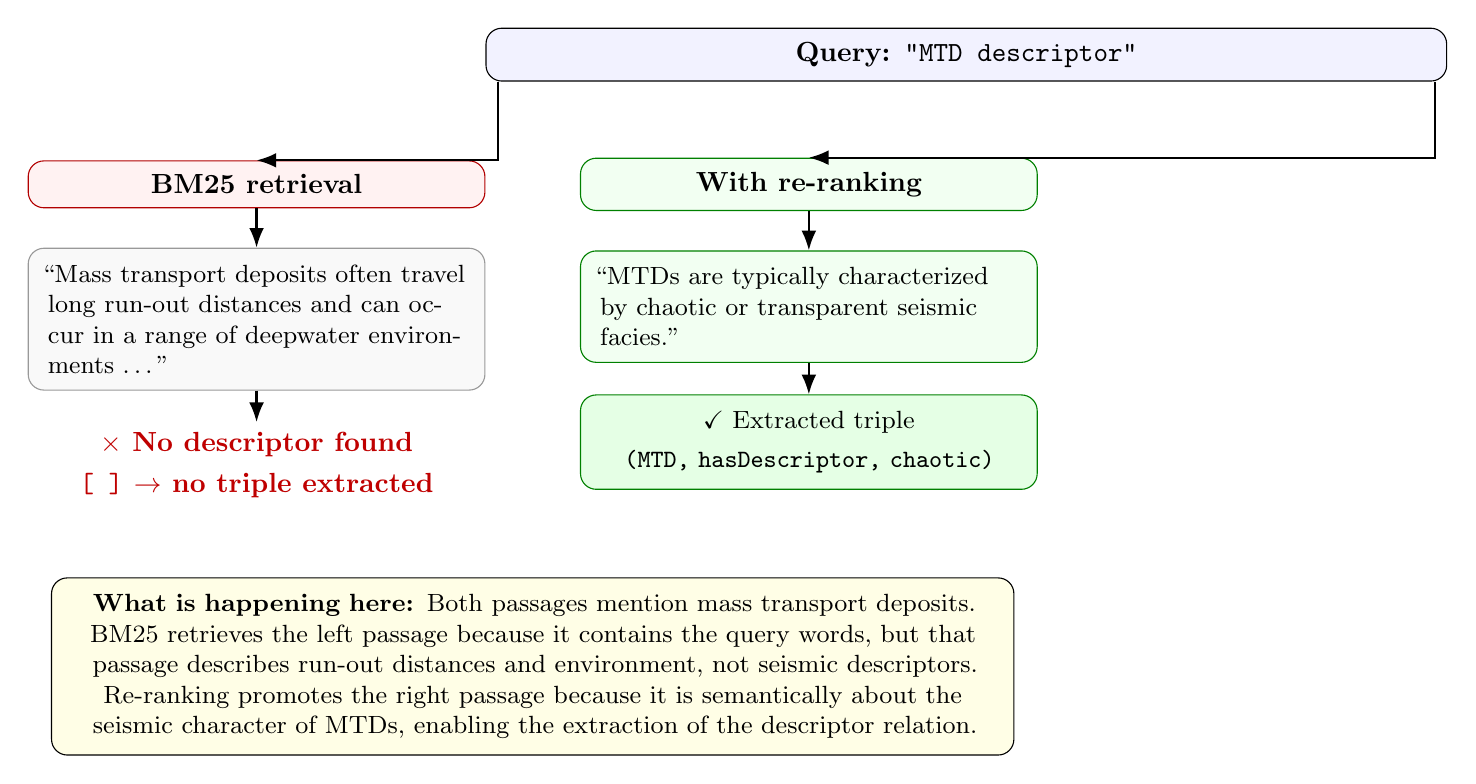
\begin{tikzpicture}[
  font=\small,
  node distance=6mm and 8mm,
  box/.style={draw, rounded corners=2mm, align=left,
      inner sep=6pt, minimum width=5.8cm},
  titlebox/.style={draw, rounded corners=2mm, align=center,
       inner sep=5pt, minimum width=5.8cm,
       font=\bfseries},
  querybox/.style={draw, rounded corners=2mm, fill=blue!5,
       align=center, inner sep=5pt,
       minimum width=12.2cm, font=\bfseries},
  bad/.style={draw=red!70!black, fill=red!5},
  good/.style={draw=green!50!black, fill=green!5},
  neutral/.style={draw=black!40, fill=gray!5},
  arrow/.style={-{Latex[length=2.5mm]}, thick}
]
\node[querybox] (query) {Query: \texttt{"MTD descriptor"}};
\node[titlebox, bad, below left=10mm and 0mm of query]
  (bm25title) {BM25 retrieval};
\node[box, neutral, below=5mm of bm25title, text width=5.3cm]
  (bm25chunk)
  {``Mass transport deposits often travel long run-out distances
  and can occur in a range of deepwater environments \ldots''};
\node[below=4mm of bm25chunk, align=center,
  text=red!75!black, font=\bfseries] (bm25out)
  {$\times$ No descriptor found\\[1mm]
 \texttt{[ ]} $\rightarrow$ no triple extracted};
\node[titlebox, good, right=12mm of bm25title] (cetitle)
  {With re-ranking};
\node[box, good, below=5mm of cetitle, text width=5.3cm]
  (cechunk)
  {``MTDs are typically characterized by chaotic or transparent
  seismic facies.''};
\node[box, draw=green!50!black, fill=green!10,
  below=4mm of cechunk, text width=5.3cm, align=center]
  (ceout)
  {\checkmark\ Extracted triple\\[1mm]
 \texttt{(MTD, hasDescriptor, chaotic)}};
\draw[arrow] (query.south west) ++(1.6mm,0) |- (bm25title.north);
\draw[arrow] (query.south east) ++(-1.6mm,0) |- (cetitle.north);
\draw[arrow] (bm25title.south) -- (bm25chunk.north);
\draw[arrow] (bm25chunk.south) -- (bm25out.north);
\draw[arrow] (cetitle.south) -- (cechunk.north);
\draw[arrow] (cechunk.south) -- (ceout.north);
\node[draw, rounded corners=2mm, fill=yellow!10,
  below=10mm of $(bm25out.south)!0.5!(ceout.south)$,
  align=center, text width=11.8cm, inner sep=6pt] (note)
  {\textbf{What is happening here:}
 Both passages mention mass transport deposits.
 BM25 retrieves the left passage because it contains the query
 words, but that passage describes run-out distances and
 environment, not seismic descriptors.
 Re-ranking promotes the right passage because it is
 semantically about the seismic character of MTDs,
 enabling the extraction of the descriptor relation.};
\end{tikzpicture}
\caption{A concrete example of retrieval failure and how re-ranking
  addresses it.
  BM25 retrieves a passage about run-out distances relevant
  to mass transport deposits in general, but useless for
  extracting a seismic descriptor.
  Re-ranking promotes a short passage that explicitly describes
  the seismic character of MTDs, making the descriptor relation
  extractable.
  This pattern BM25 retrieving topically related but
  relation-poor passages accounts for 58.2\% of failed
  queries in the BM25-only configuration.}
\label{fig:retrieval-failure}
\end{figure}

The implication for future work is that investing in better
retrieval whether through domain-adapted encoders, denser
retrieval models trained on geological text, or better query
formulation is likely to yield larger gains than increasing
the size or sophistication of the generative model.

\subsection{What Recall Against LB2019 Actually Measures}

A recall of 76.5\% against the 34-edge benchmark sounds like a
specific and interpretable number, but it requires careful
contextualisation.

The benchmark was deliberately restricted to edges that can
in principle be extracted from individual papers.
Two edges are missing from the corpus entirely, so the maximum
achievable recall is 32/34 = 94.1\%, not 100\%.
Correcting for these corpus gaps, the pipeline recovers 26 of 32
recoverable edges (81.3\%).

Beyond the corpus gaps, some of the remaining six unrecovered
edges are expressed so indirectly in the literature that no
sentence-level extraction system could be expected to recover them
without deeper semantic reasoning.
The example of \pred{pore pressure controls slope failure}  
present in 84 corpus chunks but never extracted illustrates
this: the causal chain runs through several intermediate steps
that are each stated separately across multiple sentences.

For these reasons, 76.5\% should be read as a lower bound on
what this class of system can extract from this literature, not
as a ceiling on what geological knowledge is in principle
recoverable.

\subsection{What the Verification Results Mean}

The verification results warrant careful interpretation.
The Tier-1 graph achieves 0\% not-supported triples under the
primary verifier (Qwen-7B), and independent verification with
Llama-3.1-8B confirms the result holds under a second model,
with only 4 disagreements in 100 triples.

It is important to understand what this does and does not mean.
It means that each Tier-1 triple is grounded in a source passage
that the verifier judges to support it.
It does not mean that each triple is geologically correct in an
absolute sense.
A geoscientist reading the source passages might judge some
relations to be over-attributed for example, a descriptor
might be correctly quoted from one paper but not representative
of the object class as a whole.
Independent geological validation, planned as a next step, will
characterize this kind of error.

The contribution of the verification step is not to eliminate
all error, but to make uncertainty explicit and measurable.
The tiered graph structure serves the same purpose: Tier-1 is
a conservative, high-confidence subset where each triple is
explicitly linked to a supporting sentence that can be inspected,
while Tier-2 provides broader coverage at marginally lower
confidence.


\subsection{Limitations}
\label{sec:limitations}

Several limitations bound the claims of this paper.

First, independent expert geological validation by five
domain geoscientists is underway on a stratified sample
of 29 extracted triples; results will be incorporated
in the final submitted version.
Such validation remains necessary to assess the geological correctness
of the final LLM-Rerank graph and to characterize remaining error modes
across relation types.

Second, the evaluation remains partially circular because the same
literature tradition underlies both the LB2019 ontology and the corpus
used for extraction.
The ontology nevertheless serves here as an expert benchmark rather
than as supervision labels, so the evaluation is not a training-test
leakage problem in the conventional machine-learning sense.

Third, generalization beyond the MTD sub-domain remains to be shown.
The pipeline is designed to be portable to other geological domains,
but this portability has not yet been demonstrated empirically.

Fourth, the verifier protocol provides an operational measure of
unsupported extraction, not a perfect estimate of factual correctness.
In addition, the same base model is used for both extraction and
verification, which may introduce verifier bias.
The distinction between verifier-based support and expert-judged
correctness therefore remains important in interpreting Tier-1 claims.

Fifth, the system operates on normalized text chunks and therefore
does not exploit figure captions, diagrams, or long-range document
structure, which may contain important geological evidence.

Finally, although reranking improves recall substantially, it does not
fully resolve recoverability limits imposed by ontology granularity,
corpus phrasing, and expert-synthesized relations.
The remaining unmatched benchmark edges therefore likely reflect a
combination of residual retrieval failure and genuine text-level
non-recoverability.
% ============================================================
\section{Conclusion}
\label{sec:conclusion}
% =====================================================================

We presented \method{}, an ontology-constrained retrieval-augmented
generation (RAG) pipeline for constructing geological knowledge
graphs from scientific literature using lightweight language models.
The method combines ontology-guided query generation, retrieval
grounding, LLM-based triple extraction, automated verification, and
provenance-aware graph assembly to produce literature-grounded,
evidence-traceable geological relations.

Across pipeline development, unsupported extraction decreased
substantially.
The NOT\_SUPPORTED rate fell from 78.0\% in the initial LLM
configuration to 2.9\% in the final Tier-1+2 graph, while the Tier-1 subset achieves 0\% NOT\_SUPPORTED under the
Qwen-7B verification protocol (Wilson CI: \WI{0.0}{3.6}), indicating full passage-level grounding within the verifier's criterion.
Independent cross-model verification with
Llama-3.1-8B on a stratified sample of 100 Tier-1 triples
yields $H_{T1}^{\text{Llama}} = 4.0\%$ with 96\% agreement,
indicating that the internal result should be interpreted
as a lower bound under the Qwen verification protocol.
The final reranked configuration produces a tiered knowledge graph
containing 153 triples (101 in Tier-1) and achieves 76.5\% recall
against the 34-edge LB2019 benchmark, with coverage of 10 of the
13 reference descriptors.

A central methodological result is that retrieval quality strongly
affects recoverable relation coverage in this setting.
In the BM25-only configuration, 145 of 249 ontology-guided queries
(58.2\%) produced no extracted triples because lexical retrieval often
failed to surface passages containing the relevant geological
relations.
Introducing CrossEncoder reranking increased recall from 47.1\% to
76.5\% and expanded the final graph from 103 to 153 triples while
preserving 0\% NOT\_SUPPORTED in Tier-1 under the verifier's passage-grounding criterion.
These results suggest that improvements in retrieval may be at least
as important as increases in generative model size for this type of
literature-based geological knowledge extraction.

Independent expert geological validation is still pending.
Such validation will be necessary to assess the geological correctness
of the retained relations and to identify the dominant remaining error
modes, including possible descriptor over-attribution.

Overall, these results indicate that a substantial subset of
ontology-compatible geological relations can be recovered directly
from scientific literature using an ontology-constrained RAG
pipeline.
More broadly, they suggest that future AI-assisted subsurface
interpretation systems may benefit from combining domain-aware
retrieval, structured ontologies, and explicit evidence grounding
rather than relying on language-model generation alone.

\medskip
\noindent Source code, corpus metadata, and all pipeline outputs
are available at \url{https://github.com/feriel21/ontogeorag}.

\section*{Acknowledgments}

This project is co-funded by the European Union's Horizon Europe
research and innovation programme Cofund SOUND.AI under the
Marie Sk\l{}odowska-Curie Grant Agreement No.~101081674.


\bibliographystyle{unsrtnat}
\bibliography{references}


% =====================================================================
\appendix
\section{Example Extraction Prompt}
\label{app:prompts}

The following is a representative extraction prompt
used in the \textbf{descriptor strategy}.
The prompt structure is identical across all four
query strategies; only the relation type, target
entity, and in-context examples change.

\medskip
\noindent\fbox{\parbox{0.96\linewidth}{
\small\ttfamily
\textbf{System:} You are a geological knowledge
extraction assistant. Extract structured relations
from the passages below. Return only relations that
are explicitly stated in the text.

\medskip
\textbf{Task:} Extract \texttt{hasDescriptor}
relations for the entity
\texttt{mass transport deposit}.

A \texttt{hasDescriptor} relation means: the subject
geological object is characterized by the seismic
descriptor in its internal facies or external
geometry, as stated in the text.

\medskip
\textbf{Output format:} Return a JSON list of
triples. Each triple must have fields:
\texttt{source}, \texttt{relation},
\texttt{target}. If no relation is found, return
\texttt{[]}.

\medskip
\textbf{Correct examples:}\\
\texttt{\{"source": "mass transport deposit",}\\
\texttt{ "relation": "hasDescriptor",}\\
\texttt{ "target": "chaotic"\}}\\
\texttt{\{"source": "mass transport deposit",}\\
\texttt{ "relation": "hasDescriptor",}\\
\texttt{ "target": "transparent"\}}

\medskip
\textbf{Errors to avoid:}\\
Do NOT extract: \texttt{(turbidite, hasDescriptor,
chaotic)} --- wrong subject entity.\\
Do NOT extract: \texttt{(mass transport deposit,
relatedTo, chaotic)} --- wrong relation type.\\
Do NOT infer: only extract relations explicitly
stated in the passage, not implied by geological
convention.

\medskip
\textbf{Passages:}\\
{[}retrieved passage 1{]}\\
{[}retrieved passage 2{]}\\
{[}\ldots{]}
}}

\medskip
The verification prompt presents the extracted triple
alongside its source passage and asks the model to
assign one of four verdicts:
\textsc{strong\_support}, \textsc{weak\_support},
\textsc{not\_supported}, or \textsc{skipped}, with a
one-sentence reasoning.
Complete prompt templates for all four strategies
and the verification step are available at
\url{https://github.com/feriel21/ontogeorag}.

%-------------------------------------------------------------
\section{Full Pipeline Configuration Trajectory}
\label{app:full-trajectory}

Table~\ref{tab:full-trajectory} reports all ten
pipeline configurations developed during this study.
Each configuration addresses a specific limitation
identified in the previous one.
The five configurations highlighted in the main text
(SVO-baseline, LLM-unverif., LLM-strict, LLM-BM25, LLM-Rerank) are shown in bold.
Configurations C2, C3, C6, C7, and C8 are
intermediate developmental iterations included here
for reproducibility.

\begin{table*}[htb]
\centering
\caption{Complete pipeline configuration trajectory.
  Raw = triples produced before verification.
  Retained = triples after verification and cleaning.
  $H_{T1}$ = not-supported rate in Tier-1.
  Recall against the 34-edge LB2019 benchmark.
  RE = cross-encoder re-ranking enabled.
  VP = verification policy (strict/normal).
  Configurations C2--C3 predate the dual-pass
  extraction and verification components;
  C6--C8 represent iterative refinements of
  query set and canonicalization.}
\label{tab:full-trajectory}
\small
\setlength{\tabcolsep}{4pt}
\begin{tabular}{clccccccc}
\toprule
\textbf{Config} &
\textbf{Key change} &
\textbf{RE} &
\textbf{VP} &
\textbf{Raw} &
\textbf{Retained} &
\textbf{Recall (\%)} &
\textbf{Desc.} &
$H_{T1}$ (\%) \\
\midrule
\textbf{SVO-baseline}
  & SpaCy SVO baseline
  & No & --- & 629 & 161 & 7.7 & 3/13 & n/a \\
C2
  & First Qwen-7B, no verif.
  & No & --- & -- & -- & -- & -- & -- \\
C3
  & Add schema constraints
  & No & --- & -- & -- & -- & -- & -- \\
\textbf{LLM-unverif.}
  & Add verification
  & No & normal & 242 & 137 & 65.4 & 13/13 & 78.0 \\
\textbf{LLM-strict}
  & Strict verification
  & No & strict & 106 & 20 & 19.2 & 12/13 & 0.0 \\
C6
  & Dual-pass extraction
  & No & normal & -- & -- & -- & -- & -- \\
C7
  & Add targeted queries for under-recovered relations
  & No & normal & -- & -- & -- & -- & -- \\
LLM-BM25-172q
  & Add canonicalization
  & No & normal & -- & -- & -- & -- & -- \\
\textbf{LLM-BM25}
  & Final BM25-only
  & No & normal & 534 & 103 & 47.1 & 11/13 & 0.0 \\
\textbf{LLM-Rerank}
  & Add CrossEncoder rerank
  & Yes & normal & 745 & 153 & 76.5 & 10/13 & \textbf{0.0} \\
\bottomrule
\end{tabular}
\end{table*}

\section{Full Pipeline Configuration Trajectory}
\label{app:full-trajectory}

Table~\ref{tab:full-trajectory} reports the complete
set of pipeline configurations evaluated during
development.
Metrics are reported at the per-pass level where
applicable; the final tiered KG combines both passes.
Configurations SVO-baseline through LLM-BM25-172q are developmental iterations;
LLM-BM25-172q, LLM-BM25, and LLM-Rerank are the three fully instrumented
configurations with complete per-pass statistics.

\begin{table*}[htb]
\centering
\caption{Complete pipeline configuration trajectory.
  \emph{Raw} = triples extracted before verification
  (pass A / pass B).
  \emph{Retained} = triples after verification and
  cleaning (pass A / pass B).
  \emph{Recall} = fraction of 34-edge LB2019
  benchmark recovered per pass.
  \emph{Final} = recall of the combined tiered KG.
  $H_{T1}$ = not-supported rate in Tier-1.
  \emph{Desc.} = seismic descriptor coverage
  out of 13 reference descriptors.
  RE = cross-encoder re-ranking.
  Configurations C2--C7 are developmental iterations
  for which per-pass statistics were not retained;
  key architectural changes are noted.}
\label{tab:full-trajectory}
\footnotesize
\setlength{\tabcolsep}{4pt}
\begin{tabular}{clccccccc}
\toprule
\textbf{Config} &
\textbf{Key architectural change} &
\textbf{RE} &
\textbf{Raw (A/B)} &
\textbf{Retained (A/B)} &
\textbf{Recall/pass} &
\textbf{Final recall} &
\textbf{Desc.} &
$H_{T1}$ (\%) \\
\midrule
\textbf{SVO-baseline}
  & SpaCy SVO baseline
  & No & 629/--- & 161/--- & 7.7\% & 7.7\% & 3/13 & n/a \\
C2
  & First Qwen-7B, no verification
  & No & n/r & n/r & n/r & n/r & n/r & n/r \\
C3
  & Add ontology schema constraints
  & No & n/r & n/r & n/r & n/r & n/r & n/r \\
\textbf{LLM-unverif.}
  & Add verification step
  & No & 242/--- & 137/--- & 65.4\% & 65.4\% & 13/13 & 78.0 \\
\textbf{LLM-strict}
  & Strict verification policy
  & No & 106/--- & 20/--- & 19.2\% & 19.2\% & 12/13 & 0.0 \\
C6
  & Dual-pass extraction
  & No & n/r & n/r & n/r & n/r & n/r & n/r \\
C7
  & Add targeted queries for under-recovered relations (249 total)
  & No & n/r & n/r & n/r & n/r & n/r & n/r \\
% Remplacer la ligne C8 dans le tableau par:
LLM-BM25-172q
  & Add canonicalization (172 queries)
  & No & 172/174 & 62/62 & 7/26 & 7/26 (26.9\%) & 10/13 & 0.0 \\
\textbf{LLM-BM25}
  & Expand query set to 249 (targeted query additions)
  & No & 189/186 & 71/61 & 10/34 & 16/34 (47.1\%) & 10/13 & 0.0 \\
LLM-Rerank$^*$
  & Intermediate reranking test
  & Yes & 267/248 & 82/81 & 11--12/26 & 12/26 (46.2\%) & 11/13 & 0.0 \\
\textbf{LLM-Rerank}
  & Final CrossEncoder reranking
  & Yes & 380/365 & 115/117 & 17/26 & 26/34 (76.5\%) & 10/13 & \textbf{0.0} \\
\bottomrule
\end{tabular}
\noindent\small$^*$ Metrics for C2, C3, C6, C7, and
C8 were not retained during pipeline development;
these configurations are listed for architectural
completeness. The key transitions captured by SVO-baseline,
LLM-unverif., LLM-strict, LLM-BM25, and LLM-Rerank represent the main evaluation
points reported in the main text.
\medskip
\noindent\small
n/r = not retained (intermediate configuration,
statistics not stored).
$^*$ Intermediate reranking configuration tested
before final query set expansion; not reported in
the main text.
The final recall for LLM-BM25 and LLM-Rerank exceeds the
per-pass recall because the tiered KG combines
both passes, recovering edges found in either pass.
\end{table*}

The gain from LLM-BM25-172q to LLM-BM25 (26.9\% to 47.1\%) is
attributable primarily to query set expansion
rather than to architectural changes.
C8 used 172 queries distributed across three
strategies (descriptor: 83, causal: 48,
context: 41).
LLM-BM25 expanded this to 249 queries by adding a
addition of targeted queries for under-recovered relations and increasing coverage
in the descriptor and causal categories
(descriptor: 92, causal: 56, context: 41,
spatial: 60).
This expansion accounts for the recovery of six
additional benchmark edges without any change to
the retrieval or extraction components.

\section{Benchmark Extension: Corpus-Grounding Evidence}
\label{app:bench-extension}

The evaluation benchmark was extended from 26 to 34 edges by adding
8 edges satisfying all original selection criteria
(Section~\ref{sec:benchmark}):
both entities in the geological vocabulary, relation type in the
11-type schema, and relation explicitly supported by a single cited
passage.
To verify that this extension does not introduce circularity
(i.e., that the 8 edges are grounded in the corpus independently
of the pipeline), we count the number of corpus chunks containing
both the subject and object entity for each edge.
All 8 edges co-occur in at least 4 chunks (range: 4--74),
confirming independent corpus-level support.

\begin{table}[htb]
\centering
\caption{Corpus-grounding evidence for the 8 extended benchmark
  edges. \emph{Co-occ.\ chunks} = number of the 3{,}386 corpus
  chunks containing both subject and object entities independently
  of pipeline extraction.}
\label{tab:bench-extension}
\small
\begin{tabular}{p{5.2cm}lc}
\toprule
\textbf{Edge (subject, object)} & \textbf{Relation} & \textbf{Co-occ.\ chunks} \\
\midrule
(mass transport deposit,\ low-amplitude) & \pred{hasDescriptor} & 6 \\
(mass transport deposit,\ high-amplitude) & \pred{hasDescriptor} & 4 \\
(mass transport deposit,\ continuous) & \pred{hasDescriptor} & 22 \\
(slide,\ hummocky) & \pred{hasDescriptor} & 32 \\
(submarine landslides,\ continental slope) & \pred{occursIn} & 74 \\
(megaslide,\ chaotic) & \pred{hasDescriptor} & 34 \\
(megaslide,\ transparent) & \pred{hasDescriptor} & 32 \\
(megaslide,\ layered) & \pred{hasDescriptor} & 17 \\
\bottomrule
\end{tabular}
\end{table}

\end{document}